\documentclass[tikz,border=8pt]{standalone}
\usepackage{amsmath,amssymb}
\usetikzlibrary{arrows.meta,automata,positioning,quotes}
\begin{document}
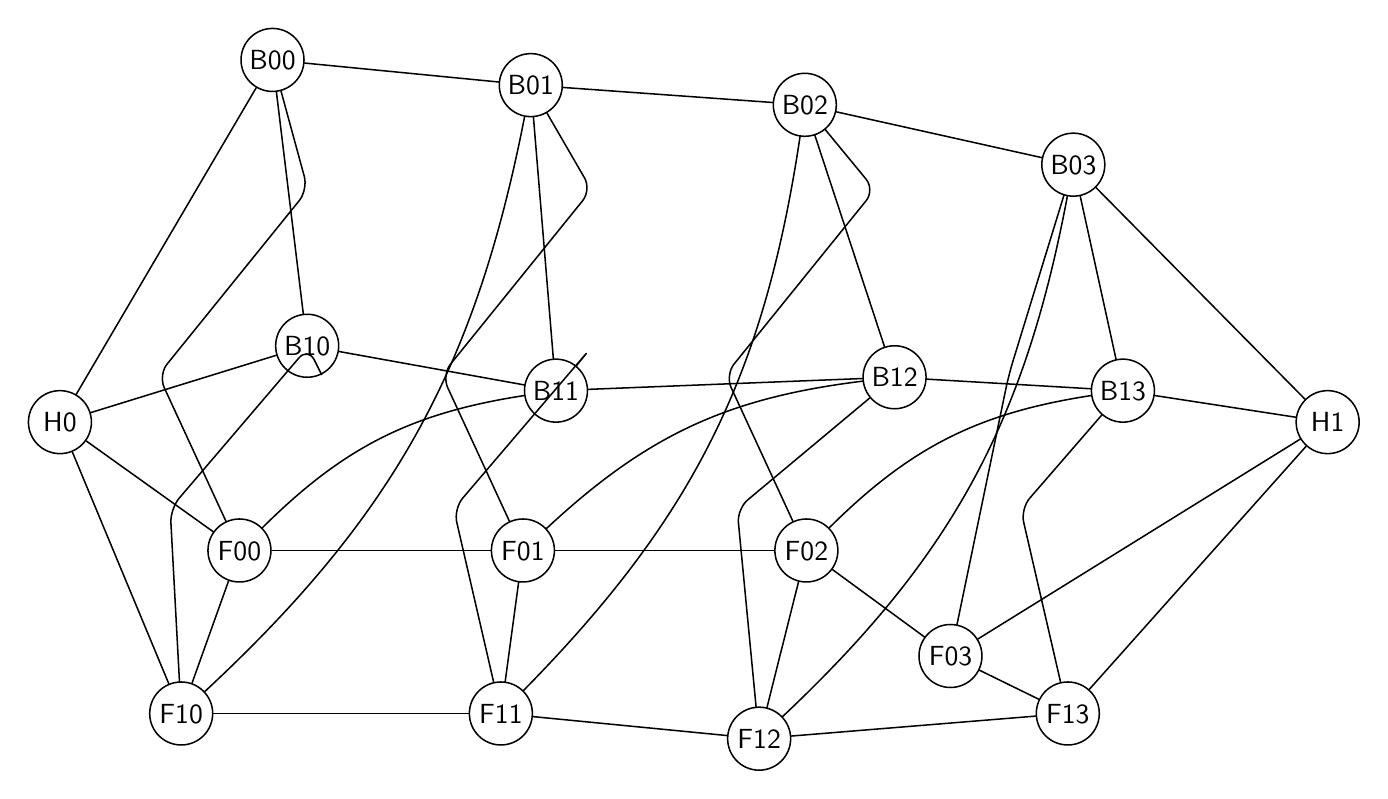
\begin{tikzpicture}[x=1cm,y=1cm]
\tikzset{
  graphnode/.style={circle,draw=black,line width=0.55pt,minimum size=8mm,inner sep=1pt,font=\sffamily},
  graphedge/.style={draw=black,line width=0.55pt,line cap=round,line join=round},
  directed/.style={graphedge,-{Stealth[length=2.4mm,width=2.0mm]}},
  undirected/.style={graphedge}
}
\node[graphnode] (n_F00) at (-5.12,-1.53) {F00};
\node[graphnode] (n_F01) at (-1.52,-1.53) {F01};
\node[graphnode] (n_F02) at (2.08,-1.53) {F02};
\node[graphnode] (n_F03) at (3.91,-2.87) {F03};
\node[graphnode] (n_F10) at (-5.86,-3.60) {F10};
\node[graphnode] (n_F11) at (-1.80,-3.60) {F11};
\node[graphnode] (n_F12) at (1.48,-3.92) {F12};
\node[graphnode] (n_F13) at (5.40,-3.60) {F13};
\node[graphnode] (n_B00) at (-4.70,4.70) {B00};
\node[graphnode] (n_B01) at (-1.42,4.38) {B01};
\node[graphnode] (n_B02) at (2.06,4.13) {B02};
\node[graphnode] (n_B03) at (5.47,3.37) {B03};
\node[graphnode] (n_B10) at (-4.26,1.07) {B10};
\node[graphnode] (n_B11) at (-1.10,0.50) {B11};
\node[graphnode] (n_B12) at (3.20,0.67) {B12};
\node[graphnode] (n_B13) at (6.10,0.50) {B13};
\node[graphnode] (n_H0) at (-7.40,0.10) {H0};
\node[graphnode] (n_H1) at (8.70,0.10) {H1};
\draw[undirected] (n_F00) -- (n_F01);
\draw[undirected] (n_F01) -- (n_F02);
\draw[undirected] (n_F02) -- (n_F03);
\draw[undirected] (n_F10) -- (n_F11);
\draw[undirected] (n_F11) -- (n_F12);
\draw[undirected] (n_F12) -- (n_F13);
\draw[undirected] (n_F00) -- (n_F10);
\draw[undirected] (n_F01) -- (n_F11);
\draw[undirected] (n_F02) -- (n_F12);
\draw[undirected] (n_F03) -- (n_F13);
\draw[undirected] (n_B00) -- (n_B01);
\draw[undirected] (n_B01) -- (n_B02);
\draw[undirected] (n_B02) -- (n_B03);
\draw[undirected] (n_B10) -- (n_B11);
\draw[undirected] (n_B11) -- (n_B12);
\draw[undirected] (n_B12) -- (n_B13);
\draw[undirected] (n_B00) -- (n_B10);
\draw[undirected] (n_B01) -- (n_B11);
\draw[undirected] (n_B02) -- (n_B12);
\draw[undirected] (n_B03) -- (n_B13);
\draw[undirected,rounded corners=5pt] (n_F00) -- (-6.15,0.70) -- (-4.25,3.05) -- (n_B00);
\draw[undirected,rounded corners=5pt] (n_F01) -- (-2.55,0.70) -- (-0.65,3.05) -- (n_B01);
\draw[undirected,rounded corners=5pt] (n_F02) -- (1.05,0.70) -- (2.95,3.05) -- (n_B02);
\draw[undirected,rounded corners=5pt] (n_F03) -- (4.65,0.70) -- (n_B03);
\draw[undirected,rounded corners=5pt] (n_F10) -- (-6.00,-1.00) -- (-4.25,1.05) -- (n_B10);
\draw[undirected,rounded corners=5pt] (n_F11) -- (-2.40,-1.00) -- (-0.65,1.05) -- (n_B11);
\draw[undirected,rounded corners=5pt] (n_F12) -- (1.20,-1.00) -- (n_B12);
\draw[undirected,rounded corners=5pt] (n_F13) -- (4.80,-1.00) -- (n_B13);
\draw[undirected] (n_F00) to[bend left=18] (n_B11);
\draw[undirected] (n_F01) to[bend left=18] (n_B12);
\draw[undirected] (n_F02) to[bend left=18] (n_B13);
\draw[undirected] (n_F10) to[bend right=18] (n_B01);
\draw[undirected] (n_F11) to[bend right=18] (n_B02);
\draw[undirected] (n_F12) to[bend right=18] (n_B03);
\draw[undirected] (n_H0) -- (n_F00);
\draw[undirected] (n_H0) -- (n_F10);
\draw[undirected] (n_H0) -- (n_B00);
\draw[undirected] (n_H0) -- (n_B10);
\draw[undirected] (n_H1) -- (n_F03);
\draw[undirected] (n_H1) -- (n_F13);
\draw[undirected] (n_H1) -- (n_B03);
\draw[undirected] (n_H1) -- (n_B13);
\end{tikzpicture}
\end{document}
